% Created 2020-04-24 vie 23:03
% Intended LaTeX compiler: pdflatex
\documentclass[12pt,a4paper, twoside]{article} % "twoside" en lugar de "twosite"
\usepackage[utf8]{inputenc}
\usepackage{pgf-umlcd}
\usepackage{lscape}
\usepackage{tikz}
\usepackage{tikz-qtree}
\usepackage{amssymb}
\usepackage{etoolbox}
\usepackage{xparse}
\usetikzlibrary{positioning, arrows.meta, shapes}
\usepackage[T1]{fontenc}
\usepackage{graphicx}
\usepackage{apalike}
\usepackage{xcolor}
\usepackage{multirow}
\usepackage{tabularx}
\usepackage{enumitem}
\usepackage{grffile}
\usepackage{longtable}
\usepackage{wrapfig}
\usepackage{rotating}
\usepackage[normalem]{ulem}
\usepackage{amsmath}
\usepackage{textcomp}
\usepackage{capt-of}
\usepackage[spanish]{babel}
\let\bibhang\relax  % Elimina la definición previa de \bibhang
\usepackage[numbers]{natbib}
\usepackage{hyperref}
\usepackage[left=2.00cm, right=2.50cm, top=2.50cm, bottom=2.00cm]{geometry}
\usepackage{fancyhdr}
\fancyhead[RO,LE]{\thepage}
\fancyhead[LO]{\emph{\uppercase{\leftmark}}}
\fancyfoot{}
\renewcommand{\headrulewidth}{1.0pt}
\pagestyle{fancy}
\date{}
\title{Testing de software en sistemas embebidos}
\hypersetup{
    pdfauthor={},
    pdftitle={Testing de software en sistemas embebidos},
    pdfkeywords={},
    pdfsubject={},
    pdfcreator={Emacs 26.2 (Org mode 9.1.9)},
    pdflang={ spanish }
}

\begin{document}

\renewcommand\refname{}
\renewcommand{\contentsname}{Tabla de contenido}
\newpage

\begin{titlepage}
    \begin{center}
        \vspace*{1cm}

                
\includegraphics[width=0.8\textwidth]{Figuras/logoFIUBA.pdf} % Ruta al logo de FIUBA

        \vspace{1.5cm}

        \textbf{\LARGE Realità : prototipo de sistema autónomo para captura de información topográfica}

        \vspace{4cm}
        \textbf{\Large Testing de software en sistemas embebidos}

        \vspace{1.5cm}


        \textbf{\Large Escrito por:}\\
        \large Karen Tatiana Zamudio

        \vspace{0.8cm}

        \textbf{\Large Revisión A}\\
        \large Esteban Volentini

        \large Mariano Finochietto

        \vfill

        \textbf{\Large Universidad de Buenos Aires}\\
        \vspace{0.2cm}

        \large 11 abril 2024

    \end{center}
\end{titlepage}
\newpage

\section*{Historial de cambios}
\label{sec:registro}

\begin{table}[ht]
  \centering
  \caption{Registro de Revisiones}
  \label{tab:registro}
  \begin{tabularx}{\linewidth}{|c|X|c|}
    \hline
    Revisión & Detalles de los cambios realizados & Fecha \\
    \hline
    0 & Creación del documento & \ 11 de abril 2024 \\
    \hline
    1 & Entrega A & \ 17 de abril 2024 \\
    \hline
  \end{tabularx}
\end{table}

\maketitle
\tableofcontents

\newpage

\section{Introducción}
\label{sec:org60390fa}

El desarrollo del trabajo Realità representa un esfuerzo colaborativo destinado a crear un sistema autónomo para la captura de información topográfica, abordando la creciente demanda de eficiencia en la obtención de datos topográficos. Como parte integral de este proceso, se presenta el Master Test Plan (MTP), una herramienta fundamental para asegurar la calidad y confiabilidad del software que respalda este innovador sistema.


\begin{figure}[htpb]
\centering
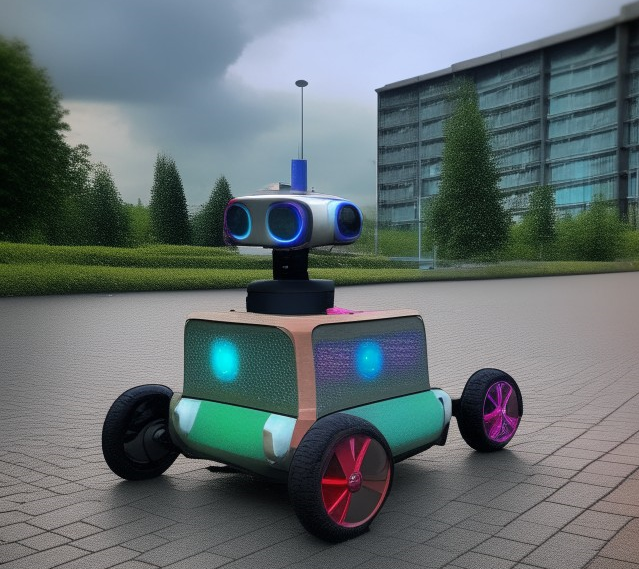
\includegraphics[width=1\textwidth]{./Figuras/Prototipo.png}
\caption{Prototipo para captura de información de nube de puntos.}
\label{fig:diagBloques}
\end{figure}

\newpage


\subsection{Propósito}
\label{sec:org434c3ef}

El objetivo principal del trabajo es abordar los desafíos relacionados con la obtención de datos topográficos precisos, por lo anterior, está dirigido a profesionales y organizaciones involucradas en proyectos que requieren información geoespacial precisa, como ingenieros, arquitectos, empresas de construcción y gestión de recursos naturales.

El prototipo se basa en la integración de múltiples sensores, que incluyen sensores GPS (Sistemas de Navegación por Satélite), sensores LIDAR (Detección y Teledetección por Luz y Alcance), un sensor de imagen con profundidad y una IMU (Unidad de Medición Inercial) en su versión inicial, los anteriores componentes trabajan en conjunto para capturar una amplia gama de datos topográficos (fusión de datos  para nube de puntos 3D), desde coordenadas geoespaciales iniciales hasta detalles visuales y altimétricos, con el potencial de escalabilidad a sensores de mayor precisión en futuras etapas del trabajo. La fusión de datos para nube de puntos 3D es una etapa clave en el proceso del sistema autónomo para captura de información topográfica. Comienza con la recopilación de datos de múltiples sensores, incluyendo GPS, LIDAR, sensor de imagen e IMU, que capturan información topográfica. Estos datos se envían al MicroControlador (MC), donde se combinan y procesan inteligentemente para generar una nube de puntos 3D con coordenada que representa el entorno topográfico, este proceso se   evidencia en la figura 2.

\begin{figure}[htpb]
\centering
\includegraphics[width=0.95\textwidth]{./Figuras/Fusión_de_Datos_para_Nube_de_Puntos_3D.pdf}
\caption{Diagrama de secuencia}
\label{fig:diagBloques}
\end{figure}




\subsection{Ámbito del sistema}
\label{sec:org12e44a1}


\subsubsection{Nombre del sistema}
\label{subsec:org12e44a2}

Se introduce con entusiasmo al innovador trabajo "Realità", un sistema autónomo diseñado para la captura de información topográfica de manera eficiente y precisa, la elección del nombre "Realità" refleja su capacidad única para capturar la realidad del entorno con una precisión excepcional. Adicionalmente, el nombre no solo simboliza la fusión de datos provenientes de múltiples sensores, como GPS, LIDAR, sensor de imagen e IMU, para crear una representación tridimensional detallada, sino que también encarna la visión de transformar sueños en una realidad tangible para quien construye este trabajo.


En un contexto donde la precisión de la información topográfica es esencial para profesionales y organizaciones en diversas áreas, "Realità" se rige como un sueño convertido en realidad, ofreciendo un enfoque revolucionario que supera los desafíos actuales y promete redefinir la manera en que se aborda la captura de datos geoespaciales.


\subsubsection{Objetivos}
\label{subsec:org12e44a2}


\begin{itemize}

\item Desarrollar un prototipo funcional del sistema autónomo para la captura de información topográfica, destacando la integración de sensores multimodales como piedra angular.

\item Demostrar la viabilidad y eficacia de esta tecnología innovadora al generar mapas precisos del entorno que sean comparables a los mapas generados por métodos tradicionales, lo que e reduce en nuevas oportunidades para la aplicación de la tecnología en una variedad de campos, como la construcción, la planificación urbana y la gestión de recursos naturales.

\item Implementar un algoritmo de fusión de datos de última generación para integrar datos de sensores GPS, LIDAR, sensor de imagen e IMU, lo anterior proporcionará una representación detallada y precisa del terreno, permitiendo a los usuarios obtener una comprensión más completa del entorno y, por ende, tomar decisiones más informadas.

\item Culminar exitosamente el desarrollo del prototipo, estableciendo así las bases para futuras mejoras y desarrollos en la captura de datos topográficos, esta plataforma experimental permitirá a los investigadores explorar nuevas tecnologías que mejoren la precisión, eficiencia y utilidad de la captura de datos topográficos.
\end{itemize}





\subsubsection{Alcance}
\label{subsec:org12e44a2}


Este trabajo tiene como alcance principal el desarrollo de un prototipo funcional para un sistema autónomo diseñado específicamente para la captura de información topográfica, la esencia del enfoque radicará en la integración de sensores multimodales, como GPS, LIDAR, sensor de imagen e IMU, con el propósito de demostrar la viabilidad y eficacia en la generación de mapas precisos del entorno, ademas la implementación de un algoritmo de fusión de datos de última generación será crucial para proporcionar una representación detallada y precisa del terreno. Todo lo anterior, llevará a cabo una evaluación exhaustiva en campos como la construcción, planificación urbana y gestión de recursos naturales.

Sin embargo, es esencial señalar que este trabajo no contemplará la implementación de sensores de mayor precisión en futuras etapas, ni explorará la integración de tecnologías aún no desarrolladas. Además, no se abordarán aspectos relacionados con la seguridad cibernética de los datos recopilados, quedando este tema claramente fuera del alcance del presente trabajo. Estas limitaciones se establecen con el propósito de proporcionar claridad con respecto a las fronteras del trabajo y dirigir futuras investigaciones hacia objetivos específicos.


\section{State transition testing}
\label{sec:orgc1c4017}

\subsection{Definición de State Transition Testing}
\label{sec:orgdaca22c}



El State Transition Testing (Pruebas de Transición de Estados) es una técnica de diseño de pruebas utilizada para evaluar el comportamiento de un sistema basado en estados. Este enfoque se centra en verificar si las transiciones entre diferentes estados del sistema se realizan correctamente de acuerdo con las especificaciones establecidas. En términos simples, un sistema basado en estados puede estar en uno de varios estados en un momento dado, y las transiciones ocurren cuando el sistema cambia de un estado a otro en respuesta a eventos específicos. Por ejemplo, en un sistema de reserva de vuelos, los estados podrían incluir disponible, reservado y cancelado, y las transiciones podrían ser reservar vuelo o cancelar reserva.


La técnica de State Transition Testing se utiliza para identificar y probar todas las posibles transiciones entre estados, así como para verificar la lógica asociada con esas transiciones. Esto garantiza que el sistema se comporte correctamente en diferentes situaciones y que los usuarios obtengan resultados esperados en todas las interacciones.

\subsection{Importancia del State Transition Testing en Realità}
\label{sec:orgdaca22c}

El State Transition Testing (STT) es una técnica de prueba de software que se puede aplicar para verificar el correcto funcionamiento del sistema Realità. El STT se basa en la definición de un modelo de estado del sistema, que describe los diferentes estados en los que puede encontrarse el sistema y las transiciones entre esos estados. Cada transición se desencadena por un evento específico y tiene como resultado un nuevo estado del sistema, para aplicar el STT al sistema Realità, se deben seguir los siguientes pasos:

\begin{enumerate}
\item Definir el modelo de estado del sistema implica identificar los diferentes estados en los que puede encontrarse el sistema, así como los eventos que desencadenan las transiciones entre esos estados.

\item Diseñar casos de prueba para cada transición, cada caso de prueba debe verificar que la transición se comporta correctamente, es decir, que el sistema pasa al estado correcto después de que se produce el evento.

\item Ejecutar los casos de prueba y analizar los resultados. Si un caso de prueba falla, indica que hay un error en el sistema que debe corregirse.


\end{enumerate}



El STT puede ser una herramienta valiosa para garantizar el correcto funcionamiento del sistema Realità. Al verificar que el sistema se comporta como se espera en todos los estados posibles, se puede reducir el riesgo de errores y garantizar que el sistema pueda capturar información topográfica de manera precisa y eficiente.


\section{Aplicación del State Transition Testing en Realità}
\label{sec:orgc1c4017}



El State Transition Testing (Pruebas de Transición de Estados) es una técnica de diseño de pruebas utilizada para evaluar el comportamiento de un sistema basado en estados. En este caso, aplicaremos esta técnica a Realità para garantizar su correcto funcionamiento y conformidad con las especificaciones establecidas.



\subsection{Identificación de los estados del sistema}
\label{sec:orgdaca22c}

El sistema Realità, al ser un sistema autónomo para la captura de información topográfica, presenta diversos estados durante su funcionamiento. Para una mejor comprensión del sistema, se detallan a continuación los estados principales:

\begin{enumerate}

\item Estado de Inicio:

\begin{enumerate}
    \item El sistema se encuentra inactivo, a la espera de instrucciones.
    \item Los sensores están desactivados y no se está capturando información.
    \item El sistema espera la interacción del usuario para iniciar el proceso de captura.
\end{enumerate}

\item Estado de configuración:

\begin{enumerate}
    \item Se configuran los parámetros de operación de cada sensor, como la frecuencia de muestreo, la resolución y el rango de medición, de acuerdo con las características del área de captura y los requerimientos del usuario.

    \item El sistema valida los parámetros ingresados y se prepara para la captura.
\end{enumerate}

\item Estado de captura:

\begin{enumerate}

    \item Se realiza la calibración interna de los sensores para garantizar la precisión y confiabilidad de las mediciones.
     \item Los sensores comienzan a capturar datos de forma simultánea, registrando mediciones de su respectiva naturaleza.

\end{enumerate}

\item Estado de procesamiento:

\begin{enumerate}
    \item El sistema fusiona los datos de los diferentes sensores en tiempo real.
    \item Los datos capturados se procesan y analizan para generar un mapa topográfico preciso.
    \item Se identifican y clasifican los elementos del entorno, como edificios, calles y vegetación.
    \item Se generan metadatos que describen el mapa y las condiciones de captura.
\end{enumerate}

\item Estado de finalización:

\begin{enumerate}
    \item La captura de datos y el procesamiento finalizan.
    \item El sistema presenta al usuario el mapa topográfico generado, junto con los metadatos correspondientes.
    \item El usuario puede guardar el mapa y los metadatos para su posterior uso.
\end{enumerate}

\item Estado de error:

\begin{enumerate}
    \item El sistema entra en este estado si se produce un error durante la captura, el procesamiento o la finalización del proceso.
    \item Se registra el tipo de error y la causa probable.
    \item El usuario es notificado sobre el error y se le proporcionan instrucciones para resolverlo.
\end{enumerate}

\end{enumerate}

\subsection{Definición de los eventos}
\label{sec:descripcion-general}

En el sistema Realità, los eventos que desencadenan las transiciones entre los diferentes estados son acciones o situaciones específicas que determinan el cambio de estado del sistema. Estos eventos pueden ser generados por el usuario, por los sensores o por el propio sistema como resultado de su funcionamiento.

A continuación, se detalla la lista de eventos que desencadenan cada estado:

\begin{enumerate}

\item Estado de inicio:
\begin{enumerate}
    \item Evento de inicio: el usuario enciende el sistema o inicia una nueva sesión de captura.
\end{enumerate}

\item Estado de configuración:
\begin{enumerate}
    \item Evento de inicio de configuración: el usuario accede al menú de configuración del sistema.
    \item Evento de modificación de parámetros: el usuario modifica los parámetros de captura, como el área de interés, la resolución deseada o el tipo de sensores a utilizar.
    \item Evento de validación de parámetros: el sistema valida los parámetros ingresados por el usuario.
    \item Evento de preparación para la captura: el sistema se prepara para iniciar la captura de datos de acuerdo con los parámetros configurados.
\end{enumerate}

\item Estado de captura:

\begin{enumerate}
    \item Evento de inicio de captura: el usuario da la orden de iniciar la captura de datos.
    \item Evento de activación de sensores: los sensores se activan y comienzan a capturar datos.
    \item Evento de calibración interna: se realiza la calibración interna de los sensores para garantizar la precisión y confiabilidad de las mediciones.
    \item Evento de captura de datos: los sensores capturan datos de forma simultánea, registrando mediciones de su respectiva naturaleza.
    \item Evento de fusión de datos en tiempo real: el sistema fusiona los datos de los diferentes sensores en tiempo real.
\end{enumerate}

\item Estado de procesamiento:
\begin{enumerate}
    \item Evento de finalización de captura: se alcanza el área de captura definida o se agota el tiempo de captura.
    \item Evento de inicio de procesamiento: los datos capturados están listos para ser procesados.
    \item Evento de procesamiento de datos: el sistema procesa y analiza los datos capturados para generar un mapa topográfico preciso.
    \item Evento de identificación y clasificación de elementos: se identifican y clasifican los elementos del entorno, como edificios, calles y vegetación.
    \item Evento de generación de metadatos: se generan metadatos que describen el mapa y las condiciones de captura.
\end{enumerate}

\item Estado de finalización:
\begin{enumerate}
    \item Evento de finalización de procesamiento: el procesamiento de datos finaliza y el mapa topográfico está generado.
    \item Evento de presentación del mapa: el sistema presenta al usuario el mapa topográfico generado, junto con los metadatos correspondientes.
    \item Evento de guardado del mapa: el usuario guarda el mapa y los metadatos para su posterior uso.
\end{enumerate}

\item Estado de error:
\begin{enumerate}
    \item Evento de detección de error: se produce un error durante la captura, el procesamiento o la finalización del proceso.
    \item Evento de registro de error: se registra el tipo de error y la causa probable.
    \item Evento de notificación de error: el usuario es notificado sobre el error y se le proporcionan instrucciones para resolverlo.
\end{enumerate}

\item Consideraciones adicionales:

\begin{enumerate}
    \item En algunos casos, un evento puede desencadenar la transición a más de un estado. Por ejemplo, el evento de detección de error puede desencadenar la transición al estado de error y al estado de finalización, dependiendo de la gravedad del error.
    \item El sistema puede incluir mecanismos de recuperación de errores para intentar resolver los errores y volver al estado anterior.
    \item La secuencia de eventos puede variar dependiendo de la configuración del sistema y las condiciones de funcionamiento.
\end{enumerate}

\end{enumerate}



\begin{table}[htbp]
\centering
\caption{Tabla de estados y eventos del sistema}
\resizebox{0.95\textwidth}{!}{%
\begin{tabular}{|p{2.5cm}|p{5cm}|p{3.5cm}|p{7cm}|}
\hline
\textbf{Estado} & \textbf{Evento} & \textbf{Siguiente Estado} & \textbf{Descripción} \\ \hline
Inicio & Inicio del sistema & Configuración & El usuario enciende el sistema o inicia una nueva sesión de captura. \\
 & Modificación de parámetros & Configuración & El usuario modifica los parámetros de captura. \\
 & Validación de parámetros & Configuración & El sistema valida los parámetros ingresados por el usuario. \\ \hline
Configuración & Preparación para la captura & Captura & El sistema se prepara para iniciar la captura de datos. \\ \hline
Captura & Inicio de captura & Captura & El usuario da la orden de iniciar la captura de datos. \\
 & Activación de sensores & Captura & Los sensores se activan y comienzan a capturar datos. \\
 & Calibración interna & Captura & Se realiza la calibración interna de los sensores. \\
 & Captura de datos & Captura & Los sensores capturan datos simultáneamente. \\
 & Fusión de datos en tiempo real & Captura & El sistema fusiona los datos de los sensores. \\
 & Finalización de captura & Procesamiento & Se alcanza el área de captura definida o se agota el tiempo de captura. \\ \hline
Procesamiento & Inicio de procesamiento & Procesamiento & Los datos capturados están listos para ser procesados. \\
 & Procesamiento de datos & Procesamiento & El sistema procesa y analiza los datos capturados. \\
 & Identificación y clasificación de elementos & Procesamiento & Se identifican y clasifican los elementos del entorno. \\
 & Generación de metadatos & Procesamiento & Se generan metadatos que describen el mapa y las condiciones de captura. \\
 & Finalización de procesamiento & Finalización & El procesamiento de datos finaliza y el mapa topográfico está generado. \\ \hline
Finalización & Presentación del mapa & Finalización & El sistema presenta al usuario el mapa topográfico generado. \\
 & Guardado del mapa & Finalización & El usuario guarda el mapa y los metadatos para su posterior uso. \\ \hline
Cualquiera & Detección de error & Error & Se produce un error durante el proceso. \\
 & Registro de error & Error & Se registra el tipo de error y la causa probable. \\
 & Notificación de error & Error & El usuario es notificado sobre el error y se le proporcionan instrucciones. \\ \hline
\end{tabular}%
}
\end{table}

\subsection{Componer el árbol de transiciones}
\label{sec:requisitos-especificos}

El árbol de transiciones es una representación visual que muestra todas las posibles transiciones entre los estados del sistema y los eventos que las desencadenan. Esta representación visual es útil para comprender mejor la estructura del sistema y diseñar casos de prueba efectivos.

Para componer el árbol de transiciones del sistema Realità, primero se identifican todos los estados y eventos. Luego, se trazan las transiciones entre ellos de acuerdo con las reglas definidas. Una vez completado el árbol de transiciones, se puede visualizar de manera clara cómo interactúan los diferentes elementos del sistema en respuesta a diversos eventos.



\subsection{Creación de casos de prueba legales}
\label{sec:requisitos-especificos}

Los casos de prueba legales son aquellos que verifican el comportamiento correcto del sistema cuando se presentan eventos válidos. Estos casos de prueba están diseñados para probar todas las transiciones permitidas entre estados y asegurarse de que el sistema responda correctamente a cada evento.

Para crear los casos de prueba legales para el sistema Realità, se identifican todos los eventos válidos y se diseñan casos de prueba específicos para cada uno de ellos. Estos casos de prueba deben cubrir todas las transiciones entre estados permitidas por el sistema, verificando que el sistema se comporte según lo esperado en cada situación.


\begin{table}[htbp]
    \centering
    \caption{Casos de prueba para Realità}
    \label{tab:casos_prueba}
    \resizebox{\textwidth}{!}{%
    \begin{tabular}{|c|c|c|c|c|c|}
    \hline
    \textbf{ID} & \textbf{Evento} & \textbf{Guardia} & \textbf{Acción} & \textbf{Estado Inicial} & \textbf{Resultado Esperado} \\
    \hline
    1 & Inicio del sistema & - & - & Inicio & Configuración \\
    \hline
    2 & Modificación de parámetros & - & - & Configuración & Configuración \\
    \hline
    3 & Validación de parámetros & - & - & Configuración & Preparación para la captura \\
    \hline
    4 & Inicio de captura & - & - & Captura & Captura \\
    \hline
    5 & Activación de sensores & Sensores activos & - & Captura & Captura \\
    \hline
    6 & Calibración interna & Sensores calibrados & - & Captura & Captura \\
    \hline
    7 & Captura de datos & Datos capturados & - & Captura & Captura \\
    \hline
    8 & Fusión de datos en tiempo real & Datos fusionados & - & Captura & Procesamiento \\
    \hline
    9 & Inicio de procesamiento & Procesamiento iniciado & - & Procesamiento & Procesamiento \\
    \hline
    10 & Procesamiento de datos & Datos procesados & - & Procesamiento & Procesamiento \\
    \hline
    11 & Identificación y clasificación de elementos & Elementos identificados & - & Procesamiento & Procesamiento \\
    \hline
    12 & Generación de metadatos & Metadatos generados & - & Procesamiento & Procesamiento \\
    \hline
    13 & Finalización de procesamiento & Procesamiento finalizado & - & Procesamiento & Finalización \\
    \hline
    14 & Presentación del mapa & Mapa presentado & - & Finalización & Finalización \\
    \hline
    15 & Guardado del mapa & Mapa guardado & - & Finalización & Finalización \\
    \hline
    16 & Detección de error & Error detectado & - & Finalización & Error \\
    \hline
    \end{tabular}
    }
\end{table}

\subsection{Creación de casos de prueba ilegales}
\label{sec:requisitos-especificos}

Los casos de prueba ilegales son aquellos que prueban el comportamiento del sistema cuando se presentan eventos inválidos o inesperados. Estos casos de prueba están diseñados para evaluar cómo el sistema maneja situaciones incorrectas y asegurarse de que responda de manera adecuada, como mostrar mensajes de error o tomar medidas correctivas.

Para crear los casos de prueba ilegales para el sistema Realità, se identifican eventos que podrían causar transiciones no permitidas entre estados o situaciones incoherentes en el sistema. Luego se diseñan casos de prueba específicos para estos eventos, verificando que el sistema maneje adecuadamente estas condiciones inesperadas.

\begin{table}[htbp]
    \centering
    \caption{Casos de prueba ilegales para Realità}
    \label{tab:casos_prueba_ilegales}
    \resizebox{\textwidth}{!}{%
    \begin{tabular}{|c|c|c|c|c|}
    \hline
    \textbf{No.} & \textbf{Configuración} & \textbf{Estado} & \textbf{Evento} & \textbf{Resultado} \\
    \hline
    1 & - & Inicio & Modificación de parámetros & Error \\
    \hline
    2 & Configuración & Captura & Inicio de captura & Error \\
    \hline
    3 & Captura & Procesamiento & Inicio de procesamiento & Error \\
    \hline
    4 & Procesamiento & Finalización & Presentación del mapa & Error \\
    \hline
    \end{tabular}
    }
\end{table}


\subsection{Creación de casos de prueba para los guardias}
\label{sec:requisitos-especificos}

Los casos de prueba para los guardias son aquellos diseñados para evaluar las condiciones de seguridad y protección del sistema. Estos casos de prueba se centran en verificar que el sistema Realità pueda detectar y responder adecuadamente a situaciones de seguridad, como intentos de acceso no autorizado o manipulación maliciosa de datos.

Para crear los casos de prueba para los guardias en el sistema Realità, se identifican posibles vulnerabilidades o amenazas de seguridad y se diseñan casos de prueba específicos para evaluar la capacidad del sistema para detectar y mitigar estas amenazas. Esto puede incluir pruebas de autenticación de usuarios, cifrado de datos, detección de intrusiones y otras medidas de seguridad.


\begin{table}[htbp]
    \centering
    \caption{Casos de prueba para la detección de errores}
    \label{tab:casos_prueba_errores}
    \begin{tabular}{|c|c|c|c|p{5cm}|}
    \hline
    \textbf{No.} & \textbf{Estado Inicial} & \textbf{Evento} & \textbf{Estado Siguiente} & \textbf{Descripción del Caso de Prueba} \\
    \hline
    1 & Inicio & Detección de error & Error & Verificar que el sistema maneje correctamente la detección de un error al iniciar. \\
    \hline
    2 & Configuración & Registro de error & Error & Verificar que el sistema registre adecuadamente un error durante la configuración. \\
    \hline
    3 & Captura & Detección de error & Error & Verificar que el sistema maneje correctamente la detección de un error durante la captura. \\
    \hline
    4 & Procesamiento & Detección de error & Error & Verificar que el sistema maneje adecuadamente la detección de un error durante el procesamiento. \\
    \hline
    5 & Finalización & Detección de error & Error & Verificar que el sistema maneje correctamente la detección de un error durante la finalización. \\
    \hline
    \end{tabular}
\end{table}


\section{Bases del test}
\label{sec:orgc1c4017}

Esta sección proporciona una visión general del proyecto, incluyendo los siguientes aspectos:


\subsection{Especificaciones del producto}
\subsubsection{Diseño funcional general}

El diseño funcional general ofrece una descripción panorámica de las funciones clave del producto, abordando sus características y capacidades fundamentales.

\subsubsection{Diseño funcional detallado}

Este documento detallado presenta una visión a profundidad de las funciones específicas del producto, proporcionando información pormenorizada sobre su implementación y operación.

\subsubsection{Guía del usuario Realità}

La guía del usuario Realità se presenta como un manual exhaustivo destinado a los usuarios finales, contiene instrucciones detalladas para aprovechar al máximo las capacidades del producto, garantizando una experiencia de usuario óptima.

\subsection{Normas}
\subsubsection{Normas internas para productos de prueba}

Establecemos normas internas que actúan como directrices esenciales para la creación y ejecución de productos de prueba, asegurando coherencia y calidad en todo el proceso.

\subsubsection{Libro Testing Embedded Software}

Este libro representa una fuente de referencia esencial que aborda las mejores prácticas en pruebas de software integrado, su contenido se utiliza como guía para garantizar un enfoque sólido y eficiente en la fase de pruebas.

\subsection{Manuales de usuario}
\subsubsection{Manual del entorno de prueba del usuario}

Este manual ofrece instrucciones detalladas sobre el entorno de prueba, proporcionando a los usuarios información clara y completa para una interacción efectiva con el sistema.

\subsubsection{Manual de herramientas de prueba del usuario}

La guía sobre las herramientas de prueba ofrece información detallada sobre las herramientas utilizadas en el proceso de prueba, asegurando una comprensión profunda de su funcionamiento y aplicación.

\subsection{Planes del proyecto}
\subsubsection{Plan de proyecto Realità}

En el plan de proyecto Realità, se detallan todos los aspectos relacionados con la gestión y ejecución del proyecto, desde los objetivos hasta la asignación de recursos, proporciona una hoja de ruta integral para el éxito del proyecto.

\subsection{Planificación}
\subsubsection{Planificación del equipo de desarrollo Realità}

La planificación detallada del equipo de desarrollo para Realità establece la estructura temporal y las tareas asignadas, garantizando una ejecución eficiente y coordinada de las actividades del equipo durante todo el proyecto.


\section{Estrategía general del test}
\label{sec:orgc1c4017}

La estrategia de pruebas de aceptación para Realità se basa en la premisa de que las pruebas de módulos y de integración son realizadas por el equipo de desarrollo. Esta estrategia se ha elaborado después de reuniones con el comisionado, líder del trabajo y gerente de pruebas específicamente para el desarrollo del trabajo Realità.


\subsection{Características de calidad y su importancia relativa}
\label{sec:org24980a8}



Subcaracterísticas seleccionadas:

\begin{enumerate}

\item Idoneidad (Suitability): verificación de que las funcionalidades e interfaces cumplan con los requisitos establecidos.

\item Operabilidad (Operability): evaluación de la interfaz de usuario en términos de simplicidad e intuición.

\item Precisión (Accurateness): mantenimiento de la precisión de los valores medidos en diversas condiciones de funcionamiento.

\item Eficiencia (Time Behaviour): garantizar que el tiempo de respuesta ante eventos críticos sea aceptable.

\item Mantenibilidad (Changeability): facilitar la actualización y adaptación del software.

\end{enumerate}

\subsection{Matriz de estrategia para Realità}
\label{sec:org24980a8}

Realità, como sistema autónomo diseñado para la captura eficiente y precisa de información topográfica, despliega diversas funciones esenciales para cumplir con los objetivos del proyecto.


\begin{table}[h]
\centering
\begin{tabular}{|l|c|c|c|c|}
    \hline
    Subsistema & Funcionalidad  & Usabilidad & Eficiencia & Mantenibilidad \\
    \hline
    SAD & ++ & ++ & + &  \\
    SP & ++ & + & ++ & + \\
    SFD3D & ++ & ++ & ++ & ++ \\
    SC & + & ++ & + & ++\\
    \hline
    Importancia relativa (100) & 40 & 20 & 25 & 15\\
    \hline
\end{tabular}
\end{table}

\subsection*{Referencias}

\begin{itemize}
    \item ++ La característica de calidad es predominante para el subsistema.
    \item + La característica de calidad es relevante para el subsistema.
    \item (vacío) La característica de calidad es insignificante para el subsistema.
\end{itemize}


A continuación, se detallan los subsistemas funcionales clave de Realità en relación con la captura de datos topográficos:

\begin{enumerate}

\item \textbf{Subsistema adquisición de datos (SAD)}
\begin{enumerate}
\item Realità emplea una variedad de sensores y controladores para garantizar una captura eficiente de datos topográficos:
\begin{itemize}
\item Sensores LiDAR: utilizados para la detección remota y la generación de modelos tridimensionales precisos del entorno.
\item Sensores GPS: proporcionan información geoespacial precisa para la localización y el mapeo del terreno.
\item Sensores de imagen con profundidad: permiten la captura de imágenes tridimensionales del entorno con información de profundidad.
\item Sensores IMU (Unidad de Medición Inercial): utilizados para medir y registrar los movimientos y la orientación del dispositivo en tiempo real.
\item Controladores de movimiento: responsables de coordinar y controlar los movimientos del dispositivo para garantizar una captura precisa y eficiente de los datos topográficos.
\end{itemize}

\end{enumerate}

Estos componentes trabajan en conjunto para proporcionar una captura de datos integral y precisa, permitiendo a Realità cumplir con sus objetivos de manera efectiva.

\item \textbf{Subsistema de procesamiento de datos (SP)}
\begin{enumerate}

\item \textbf{Microcontrolador (MC):} el microcontrolador STM32 integra toda la información de los sensores y coordina el procesamiento de datos para su posterior análisis y utilización.
\end{enumerate}

\item \textbf{Subsistema de fusión de datos 3D (SFD3D)}
\begin{enumerate}

\item \textbf{Generador de Nube de Puntos 3D:} este componente genera la nube de puntos 3D a partir de los datos fusionados, proporcionando una representación detallada del terreno topográfico.

\item \textbf{Clasificación de Puntos 3D:} este algoritmo clasifica los datos capturados por los diferentes sensores para crear una representación tridimensional precisa del entorno.
\end{enumerate}

\item \textbf{Subsistema de comunicación (SC)}
\begin{enumerate}
\item \textbf{Sensores Wi-Fi, Bluetooth y de radio:} estos sensores permiten la comunicación inalámbrica para la coordinación, manejo, inicio y finalización de la información entre Realità y otros dispositivos o estaciones base.
\end{enumerate}

\item \textbf{Integración sinérgica del sistema completo}
\begin{enumerate}
\item \textbf{Integración holística para una captura integral:} la integración completa que proporciona una solución holística, maximizando la eficiencia y precisión en la captura de datos topográficos alineados con los requerimientos del proyecto.
\end{enumerate}

\end{enumerate}


\subsection{Técnicas de diseño de pruebas}

Las técnicas de diseño de pruebas desempeñan un papel crucial en el proceso de aseguramiento de la calidad de Realità, estas técnicas proporcionan el marco fundamental para evaluar la funcionalidad, usabilidad, confiabilidad y precisión del sistema autónomo de captura de información topográfica.

En el contexto específico de Realità, las técnicas de diseño de pruebas se adaptan de manera precisa y meticulosa para abordar los desafíos únicos asociados con la integración de sensores multimodales, como GPS, LIDAR, sensor de imagen e IMU.

\subsubsection{Pruebas de funcionalidad}

\textbf{Descripción:} verificar la funcionalidad de cada componente del sistema Realità, incluyendo la captura de datos, procesamiento y generación de mapas.

\textbf{Técnicas:}
\begin{enumerate}
    \item Pruebas unitarias: evaluar cada módulo individualmente.
    \item Pruebas de integración: verificar la interacción entre módulos, especialmente en la fusión de datos de múltiples sensores.
    \item Pruebas de sistema: validar la funcionalidad del sistema en su conjunto.
\end{enumerate}

\subsubsection{Pruebas de usabilidad}

\textbf{Descripción:} evaluar la facilidad de uso del sistema Realità para los usuarios finales, centrándose en la interpretación de los mapas generados.

\textbf{Técnicas:}
\begin{enumerate}
    \item Pruebas de interfaz de usuario (UI): Evaluar la interfaz para asegurar una experiencia intuitiva.
    \item Pruebas de navegación: verificar la facilidad de movimiento y acceso a funciones clave.
\end{enumerate}

\subsubsection{Pruebas de confiabilidad}

\textbf{Descripción:} asegurarse de que Realità produce resultados precisos y consistentes bajo diversas condiciones.

\textbf{Técnicas:}
\begin{enumerate}
    \item Pruebas de estabilidad: evaluar la capacidad del sistema para manejar cargas de trabajo sostenidas.
    \item Pruebas de estrés: exponer el sistema a condiciones extremas para evaluar su comportamiento.
\end{enumerate}

\subsubsection{Pruebas de fusión de datos}

\textbf{Descripción:} garantizar que la integración de datos de sensores GPS, LIDAR, sensor de imagen e IMU genere mapas detallados y precisos.

\textbf{Técnicas:}
\begin{enumerate}
    \item Pruebas de fusión de datos 3D: evaluar la capacidad del sistema para generar representaciones tridimensionales precisas.
    \item Pruebas de coherencia de datos: verificar que los datos de diferentes sensores se integren de manera coherente.
\end{enumerate}

\subsubsection{Pruebas de captura de datos en campo}

\textbf{Descripción:} evaluar el rendimiento de Realità durante la captura de datos topográficos en situaciones del mundo real.

\textbf{Técnicas:}
\begin{enumerate}
    \item Pruebas de campo simuladas: emular condiciones del mundo real para evaluar la precisión y eficacia de la captura de datos.
\end{enumerate}


\begin{table}[h]
\centering
\begin{tabular}{|l|c|c|c|c|c|c|}
\hline
\textbf{Prueba} &\textbf{Idoneidad} & \textbf{Operabilidad} & \textbf{Precisión} & \textbf{Tiempo} & \textbf{Cambiabilidad}\\
\hline
Unitarias & & ++ & + & + & + \\
Integración & & ++ & & ++ &   \\
Sistema & & + & ++ & ++ & \\
UI & & & ++ & &\\
Navegación & & & ++ &  & \\
Estabilidad & & + & ++ &  &\\
Estrés & & + & ++ & & \\
SFD3D & ++ & ++ & ++ & ++ & \\
Coherencia  & & & ++ & &\\
Simuladas & & ++ & ++ & ++ & ++\\
\hline
\end{tabular}
\caption{Matriz de Técnicas de Diseño para Pruebas en Realità}
\label{tab:design_techniques_matrix}
\end{table}


\subsection{Esfuerzo estimado}

La estimación de esfuerzo es un componente vital en la planificación de pruebas de aceptación para el proyecto Realità, al abordar la complejidad y amplitud del sistema autónomo de captura de datos topográficos, es esencial prever y asignar recursos de manera precisa.

Esta subsección se centra en la evaluación cuidadosa de las tareas relacionadas con las pruebas, considerando factores como la magnitud de la implementación, la diversidad de las técnicas de prueba y las posibles contingencias, una estimación realista y fundamentada no solo facilita la asignación adecuada de recursos, sino que también sirve como un indicador crucial para evaluar la viabilidad temporal y financiera del proyecto Realità.

\begin{table}[h]
\centering
\begin{tabular}{|l |r|}
\hline
\textbf{Actividad} & \textbf{Esfuerzo (horas)} \\
\hline
Plan de pruebas & 20 \\
Fase de planificación y control & 80 \\
Gerencia de pruebas & 48 \\
Gerencia de configuración de pruebas & 28 \\
Soporte metodológico & 44 \\
Fase de preparación & 32 \\
Fase de especificación & 80 \\
Fase de ejecución & 200 \\
Fase de finalización & 16 \\
\hline
\textbf{Total} & \textbf{548} \\
\hline
\end{tabular}
\caption{Esfuerzo estimado para el proceso de pruebas}
\label{tab:estimated_effort}
\end{table}


\subsection{Planificación}

La planificación meticulosa es esencial para el éxito de cualquier proyecto, y las pruebas de aceptación para Realità no son la excepción, en esta fase, se delinea un camino claro que abarca desde la elaboración del plan de pruebas hasta la finalización del informe de resultados y conclusiones, cada actividad se ha calendarizado de manera estratégica para cumplir con el ambicioso objetivo de completar el proyecto dentro del periodo del 10 de marzo al 30 de junio.

Con un enfoque organizado y detallado, se busca asegurar la eficiencia y efectividad en cada etapa del proceso, contribuyendo así al desarrollo exitoso del sistema autónomo de captura de datos topográficos.

\begin{table}[h]
\centering
\begin{tabular}{|l|l|l|l|}
\hline
\textbf{Actividad} & \textbf{Inicio} & \textbf{Fin} & \textbf{Responsable} \\
\hline
Plan de pruebas & 10/03 & 19/03 & Equipo de Pruebas \\
\hline
\multicolumn{4}{|c|}{\textbf{Fase de Planificación}} \\
\hline
Elaboración del documento de plan de pruebas & 20/03 & 31/03 & Líder de Pruebas \\
Revisión del plan con el equipo & 01/04 & 09/04 & Equipo de Pruebas \\
Configuración de pruebas & 10/04 & 23/04 & Ingeniero de Configuración \\
Soporte metodológico & 24/04 & 07/05 & Especialista en Metodología \\
\hline
\multicolumn{4}{|c|}{\textbf{Fase de Preparación}} \\
\hline
Elaboración de casos de prueba & 15/03 & 31/03 & Analista de Pruebas \\
Revisión de casos de prueba & 01/04 & 03/04 & Equipo de Pruebas \\
\hline
\multicolumn{4}{|c|}{\textbf{Fase de Ejecución}} \\
\hline
Ejecución de pruebas & 10/05 & 26/05 & Equipo de Pruebas \\
\hline
\multicolumn{4}{|c|}{\textbf{Fase de Finalización}} \\
\hline
Informe de resultados y conclusiones & 27/05 & 28/05 & Líder de Pruebas \\
\hline
\end{tabular}
\caption{Planificación de Pruebas de Aceptación para \textit{Realità}}
\label{tab:planning}
\end{table}

\section{Amenazas, riesgos y medidas}

El entorno de pruebas para el proyecto Realità no está exento de desafíos potenciales y riesgos que podrían afectar el éxito de las pruebas de aceptación, por lo anterior se hace necesario identificar, evaluar y gestionar estas amenazas de manera proactiva garantizado la integridad y la eficacia del proceso de prueba.

En esta subsección, se abordarán posibles amenazas y riesgos, desde limitaciones tecnológicas hasta cambios inesperados en los requisitos, y se propondrán medidas mitigadoras específicas.

\begin{enumerate}
  \item Posible retraso en la entrega a prueba: en caso de retrasos, se utilizará la estrategia de prueba para determinar las pruebas omitidas, asegurando una cobertura adecuada incluso bajo restricciones de tiempo.
  \item Equipo de desarrollo disuelto después de la entrega: se garantizará la presencia de al menos un desarrollador experimentado durante la ejecución de pruebas para abordar cualquier problema inesperado y mantener el conocimiento del sistema.
  \item Disponibilidad limitada del experto de dominio: se planificará de manera adecuada, anticipando posibles retrasos y asegurando la máxima disponibilidad del experto de dominio cuando sea necesario.
  \item Diseñadores trabajando en el diseño funcional y guías de usuario: se garantizará la disponibilidad oportuna de los diseñadores para mantener la coherencia y reproducibilidad en el diseño funcional y las guías de usuario.
\end{enumerate}

\section{Infraestructura}

\subsection{Entorno de pruebas}

El equipo de pruebas está compuesto por cinco personas, durante el proyecto de prueba, se debe disponer de dos (2) PC con una configuración de hardware estándar y el software estándar utilizado por Solidly Embedded Ltd. (para software especial, consulte la sección) que requiere un espacio mínimo de 20 GB en el directorio de gestión del producto.

\subsection{Herramientas de pruebas}

Las siguientes herramientas de prueba son esenciales:

\begin{enumerate}
  \item Herramienta de gestión de defectos \textit{DefectTracker}.
  \item Herramienta de gestión de cambios \textit{ChangeMaster}.
  \item Software de planificación.
  \item Hardware adicional para rastrear el comportamiento interno eferente a la captura de información topográfica.
\end{enumerate}

\subsection{Entorno}

Se utiliza el entorno de prueba estándar, los probadores utilizan su espacio de oficina y campo durante el proyecto de prueba.

\section{Organización de pruebas}

\subsection{Roles de pruebas}

Los siguientes roles de prueba son necesarios en este proyecto:

\begin{enumerate}
  \item Ingeniero de pruebas.
  \item Gerente de pruebas.
  \item Soporte metodológico.
  \item Soporte técnico.
  \item Experto en dominio.
  \item Gerente de configuración de pruebas.
\end{enumerate}


\subsection{Personal de Pruebas}

\begin{table}[h]
\centering
\begin{tabular}{|l |l |l|}
\hline
\textbf{Función} & \textbf{Nombre} & \textbf{Equivalente a Tiempo Completo} \\
\hline
Gerente de Pruebas & T. Testware & 0.20 \\
Probador & P. Testcase & 1.00 \\
Probador & F. Testscript & 1.00 \\
Soporte & G. Allround & 1.00 \\
Experto en Dominio & A. Experto & 0.60 (durante la ejecución de pruebas) \\
\hline
\end{tabular}
\caption{Funciones y equivalente a tiempo completo del personal de pruebas}
\label{tab:test_staff}
\end{table}


\section{Entregables de pruebas}

\subsection{Documentación del proyecto}

Se producirán los siguientes documentos durante el proyecto de prueba:

\begin{enumerate}
  \item Plan de pruebas: el documento inicial y todas sus versiones anteriores/futuras.
  \item Informes de defectos: se informan todos los defectos observados.
  \item Informes semanales: informes de progreso realizados por el gerente de pruebas.
  \item Recomendación para la liberación: formalmente es el final de la fase de ejecución de pruebas.
  \item Informe de revisión: este informe da una evaluación del proceso de pruebas durante el proyecto.
\end{enumerate}

\subsection{Testware}

Los siguientes documentos son entregables del proyecto de prueba:

\begin{enumerate}
  \item Guion de pruebas: una descripción de cómo se realiza la prueba. Contiene acciones y verificaciones, relacionadas con casos de prueba, indicando la secuencia de ejecución.
  \item Escenario de pruebas: un micro-plan de pruebas que coordina la ejecución de varios guiones de prueba y asigna probadores a los guiones de prueba.
  \item Conjunto de datos inicial: archivos y conjuntos de datos necesarios para iniciar ciertas pruebas.
\end{enumerate}

\subsection{Almacenamiento}

La estructura de directorios mostrada en la Tabla \ref{tab:directory_structure} está implementada en el servidor central de Solidly Embedded Ltd, el directorio se almacena en el directorio de gestión de productos: \texttt{\textbackslash\textbackslash PROD\_MANAG}.

\begin{table}[h]
\centering
\begin{tabular}{|l| l|}
\hline
\textbf{Directorio} & \textbf{Contenido} \\
\hline
\texttt{ACC\_TEST\_REALITA} & Directorio principal del proyecto \\
\texttt{PROCDOC} & Documentación del proyecto \\
\texttt{WORK\_TESTWARE} & Directorio de trabajo para testware \\
\texttt{FINAL\_TESTWARE} & Directorio para archivar testware \\
\texttt{DEFECTS} & Base de datos para el almacenamiento de defectos \\
\texttt{OTHER} & Todos los demás documentos utilizados o producidos \\
\hline
\end{tabular}
\caption{Estructura de directorios}
\label{tab:directory_structure}
\end{table}

\section{Gestión de configuración}

\subsection{Control del proceso de pruebas}

El progreso de las pruebas y el agotamiento del presupuesto y el tiempo se monitorean y informan durante el proyecto de pruebas. Esto se realiza semanalmente y los resultados se informan en la reunión semanal de progreso.

\subsection{Gestión de defectos}

Para la gestión de defectos, se utiliza la herramienta "DefectTracker", se sigue el procedimiento estándar de defectos (SolEmb 76.1 "Procedimiento de defectos").

\subsection{Métricas}

El jefe de pruebas realiza un seguimiento de las siguientes métricas:

\begin{enumerate}
    \item Número de defectos abiertos por categoría de gravedad en un momento dado.
    \item Número de defectos resueltos en un período por categoría de gravedad.
    \item Número total de defectos detectados.
    \item Número de retrabajos por defecto.
    \item Número total de retrabajos.
\end{enumerate}

\subsection{Ítems de gestión de configuración}

El plan de pruebas está sujeto a la gestión de configuración, comenzando con la primera versión completa. El resto del testware se somete a la gestión de configuración después de la fase de finalización. Los cambios en la infraestructura de pruebas están sujetos a la gestión de configuración del departamento de soporte técnico de Solidly Embedded Ltd.



\newpage


\section{Bibliografía}

\begin{enumerate}
      \item Bart Broekman, Edwin Notenboom. \emph{Testing Embedded Software}. Addison-Wesley Professional, 2003. ISBN: 978-0201795238
  % Agrega más referencias según sea necesario
\end{enumerate}



\end{document}
